\documentclass[8pt]{beamer}

\mode<presentation>
{
  \usetheme{Warsaw}       % or try default, Darmstadt, Warsaw, ...
  \usecolortheme{dolphin} % or try albatross, beaver, crane, ...
  \usefonttheme{serif}    % or try default, structurebold, ...
  \setbeamertemplate{navigation symbols}{}
  \setbeamertemplate{caption}[numbered]
} 

\usepackage[spanish]{babel}
\usepackage[utf8x]{inputenc}
\usepackage{wrapfig}
\usepackage[beamer,customcolors]{hf-tikz} %Para hacer los cuadraditos de colores en las ecuaciones.
\hfsetfillcolor{alerted text.fg!10}
\hfsetbordercolor{alerted text.fg}
\usepackage{subcaption} %Para el entorno subfiguras.
\usepackage{ragged2e} % Justificar.
\usepackage{wrapfig}


% On Overleaf, these lines give you sharper preview images.
% You might want to `comment them out before you export, though.
\usepackage{pgfpages}
\pgfpagesuselayout{resize to}[physical paper width=8in, physical paper height=6in]

% Here's where the presentation starts, with the info for the title slide
\title[Rol del Eje de Simetría Quíntuple en TrV]{\textbf{Cálculos Computacionales en Macromoléculas: Rol del Eje de Simetría Quíntuple en el Virus del Triatoma (TrV). Comparación con otros Virus Icosaédricos.}}
\author{Juan Francisco Viso}
\institute{Universidad Nacional del Sur \\ Instituto de Física del Sur}
\date{8 de Junio de 2018}

\logo{
\includegraphics[scale=0.05]{Figure/UNS.jpg}}

\begin{document}

\begin{frame}
  \titlepage
   \begin{center}
   \begin{minipage}{0.9\textwidth}
     \centering
     %\vspace{-1.2cm}
     \underline{Director} \hfill \underline{Co-Director} \\ Marcelo D. Costabel \hfill Diego Guérin
    \end{minipage}
  \end{center}
\end{frame}

\begin{frame}[t]
\justifying
\begin{wrapfigure}{r}{0.5\textwidth}
\Centering
\only<1>{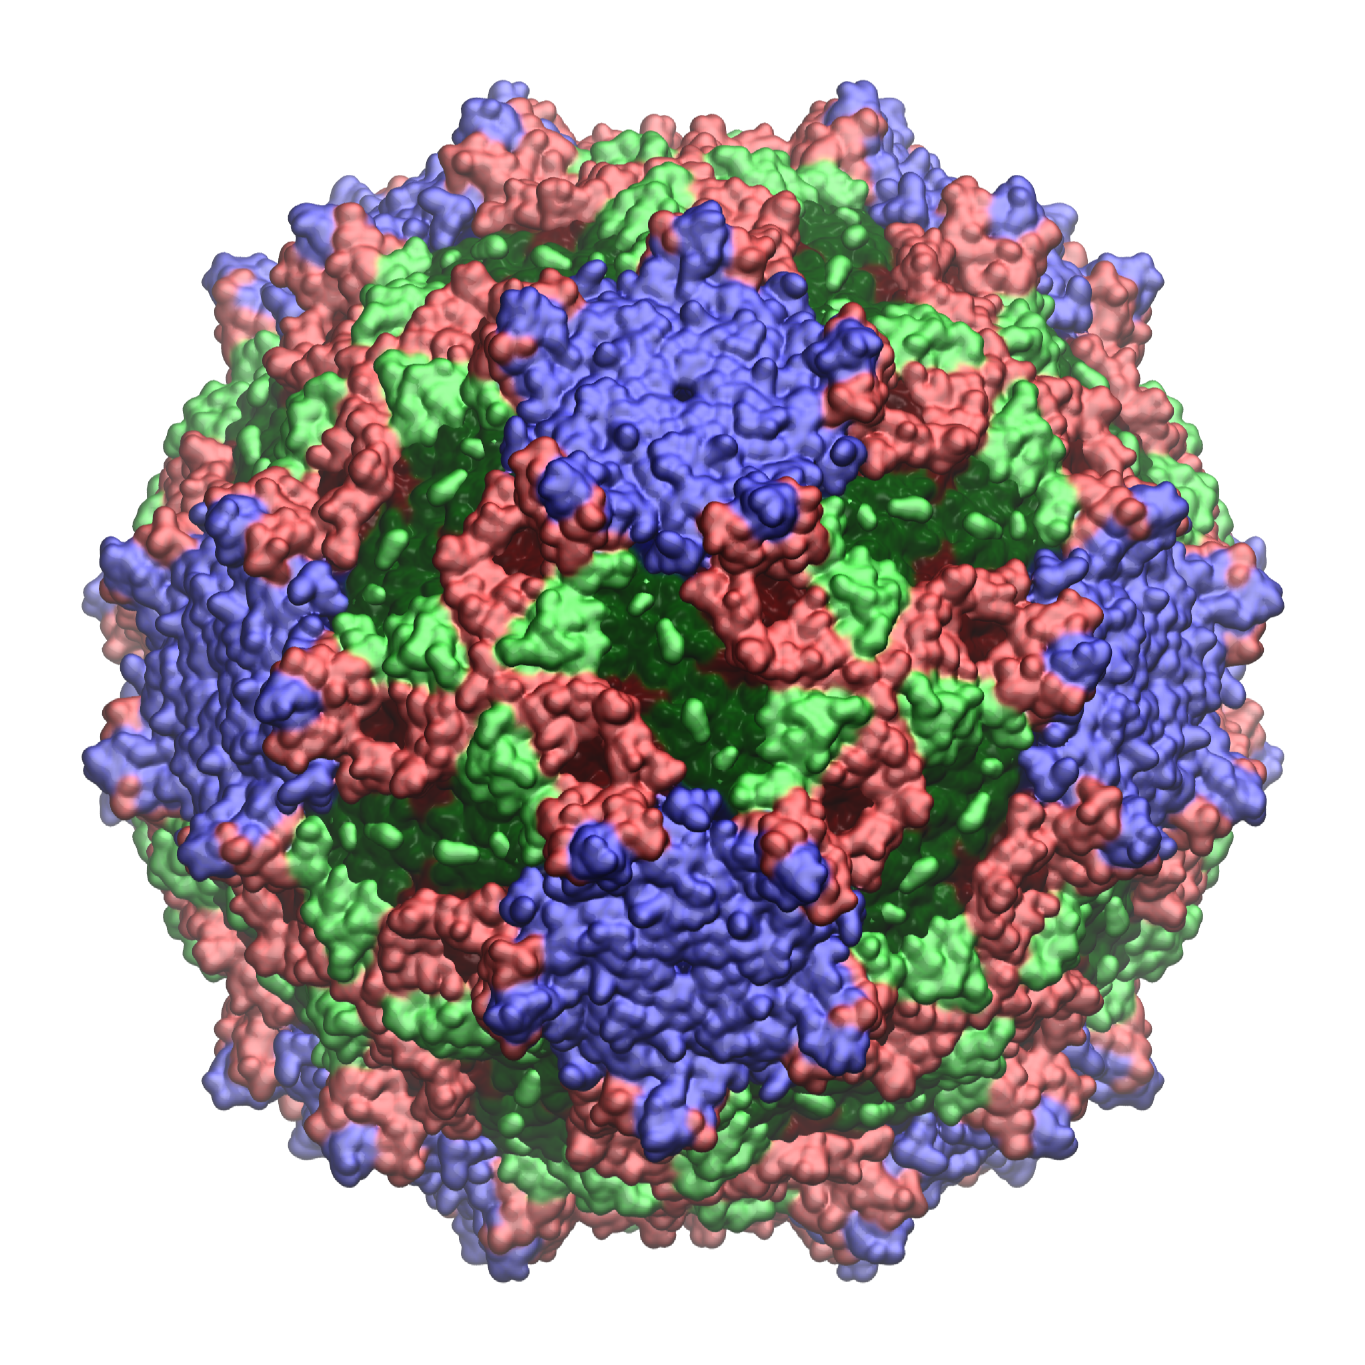
\includegraphics[width=0.5\textwidth]{Figure/TrV_Capsid.png}}
\only<2>{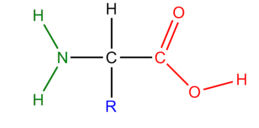
\includegraphics[width=0.3\textwidth]{Figure/aa.jpg} \\
               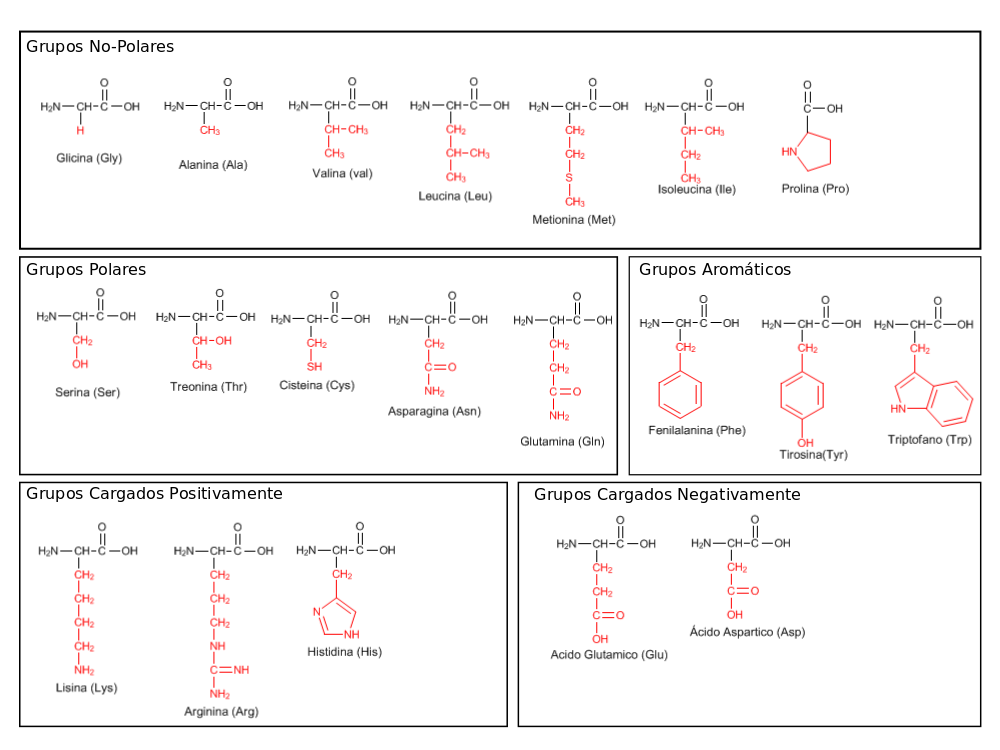
\includegraphics[width=0.5\textwidth]{Figure/aa2.png}}
\only<3>{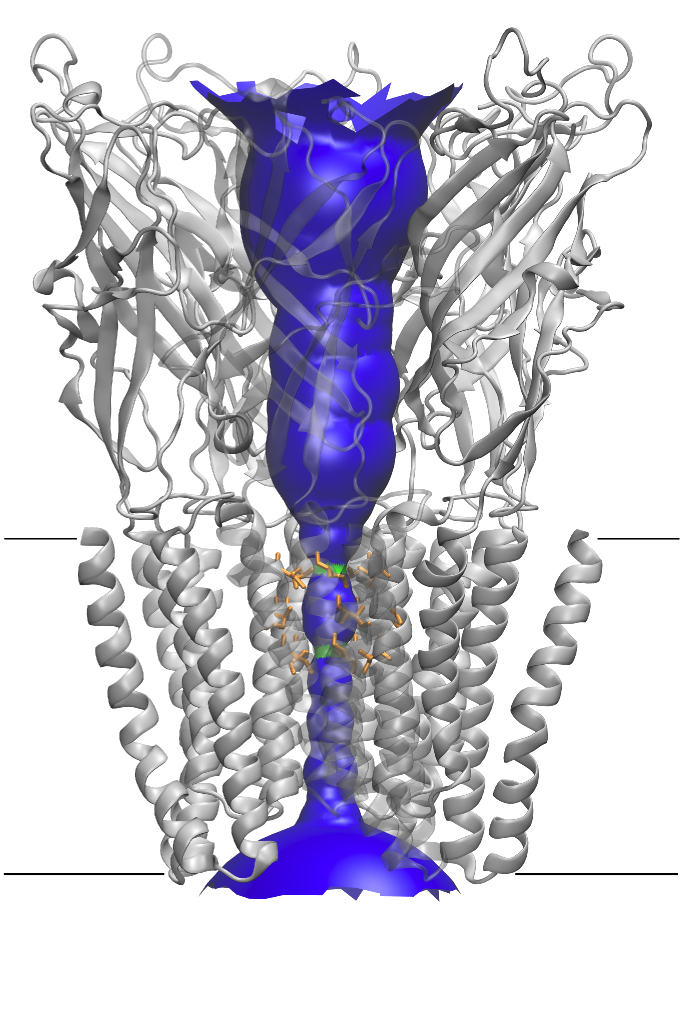
\includegraphics[width=0.5\textwidth]{Figure/GLIC.png}}
\end{wrapfigure}
$\bullet$ Las cápsides virales son estructuras proteicas cuya función consiste en proteger el material genético del virus y son las encargadas de interactuar con el medio y comenzar el proceso de infección. Sin embargo, este proceso no ha sido completamente explicado aún.

\invisible<-1>{ \vspace{0.1cm}
$\bullet$ Las proteínas son componentes químicos de las sustancias orgánicas. Estructuralmente son cadenas lineales cuyos monómeros son los aminoácidos. Los cuales están formados por un grupo amino ($-NH_2$ ), un grupo  ácido o carboxilo ($-COOH$) y un grupo (R) que varia en cada uno de los veinte aminoácidos que existen en la naturaleza.}

\invisible<-2>{ \vspace{0.1cm}
$\bullet$ Un grupo muy estudiado de proteínas, son las proteínas que interactúan con las membranas celulares, particularmente las canales iónicos. Estas proteínas presentan estructuras macromoleculares complejas cuya función es el transporte de ciertas moléculas entre el exterior y el interior de las células.}

\end{frame}

\begin{frame}[t]
%\vspace{-1cm}
\justifying
Los virus icosaédricos, como los del género Picornavirales, poseen cápsides con gran simetría. Estas cápsides poseen varios ejes de simetría dobles, triples y quíntuples. Particularmente, se ha propuesto que la cavidad presente en el eje de simetría quíntuple podría ejercer un rol como canal de iones (\textit{Susana Kalko et al.}). Sin embargo, esta hipótesis no ha sido corroborada.

\only<1>{
\begin{figure}[ht]
\centering
\hspace*{\fill}
\begin{subfigure}[t]{.46\textwidth}
  \centering
  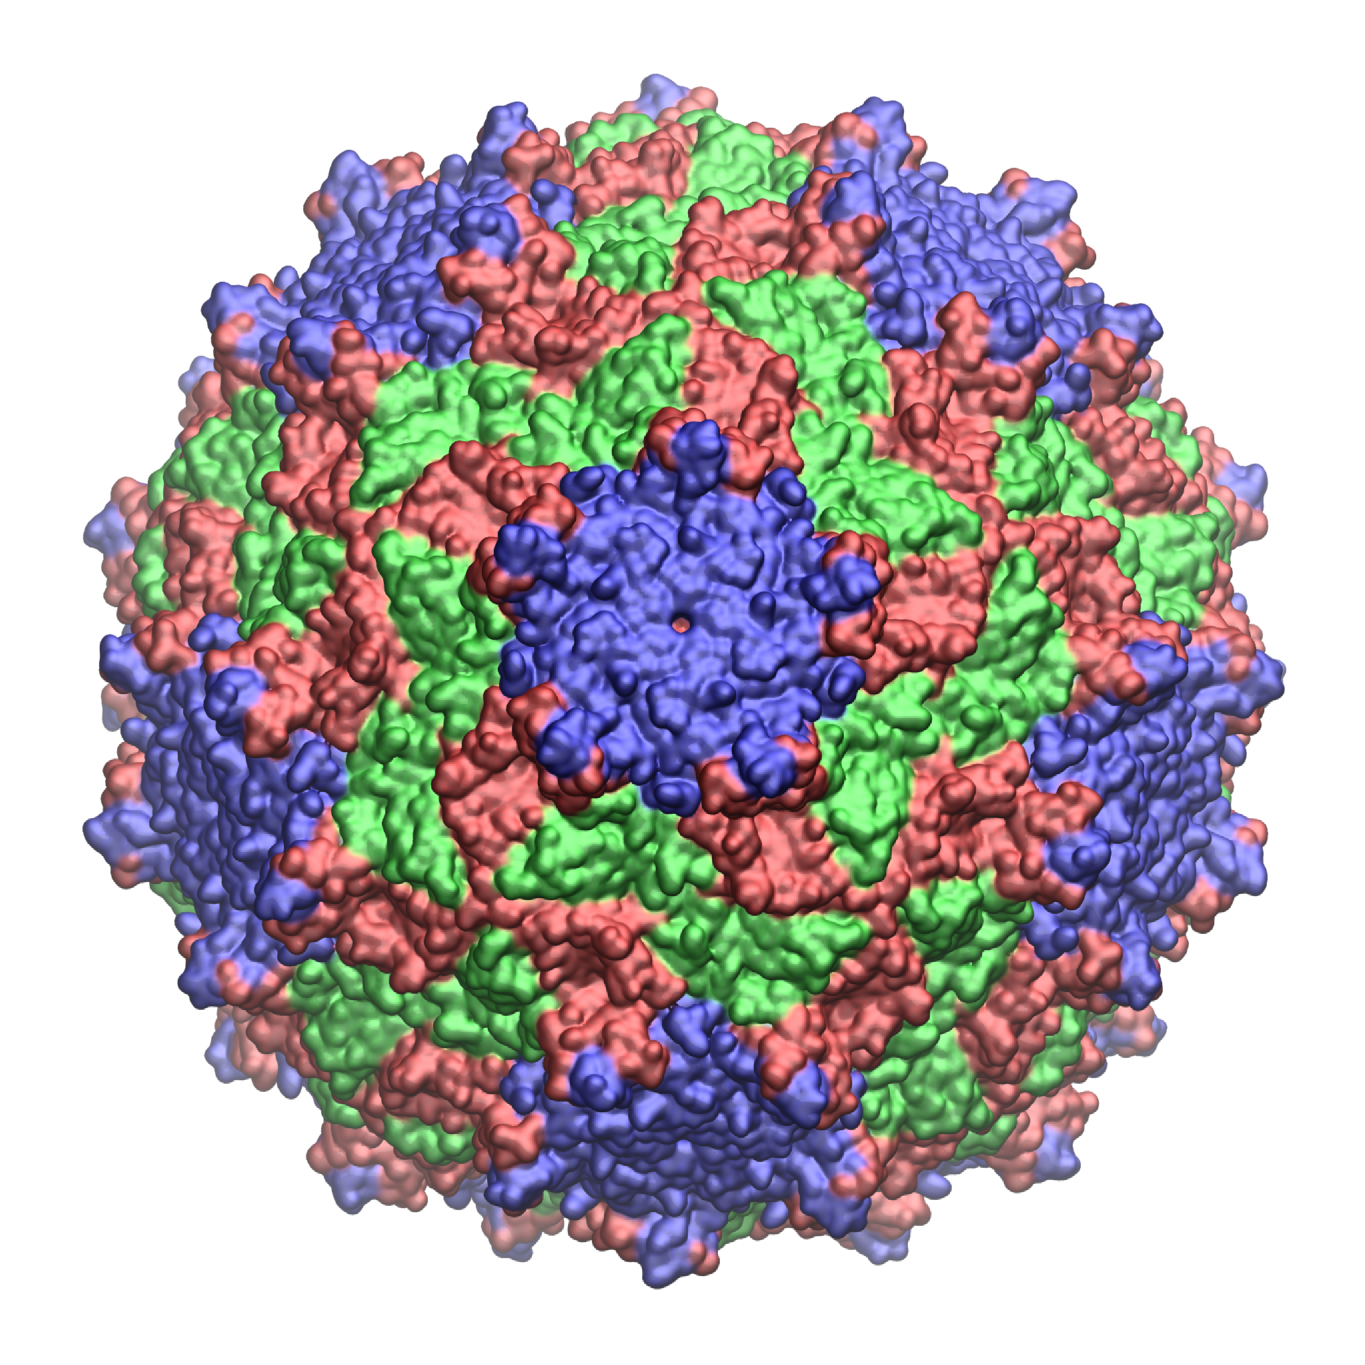
\includegraphics[width=1\textwidth]{Figure/TrV_Capsid_Ch4.png}
\end{subfigure}
\hspace*{\fill}
\begin{subfigure}[t]{.46\textwidth}
  \centering
  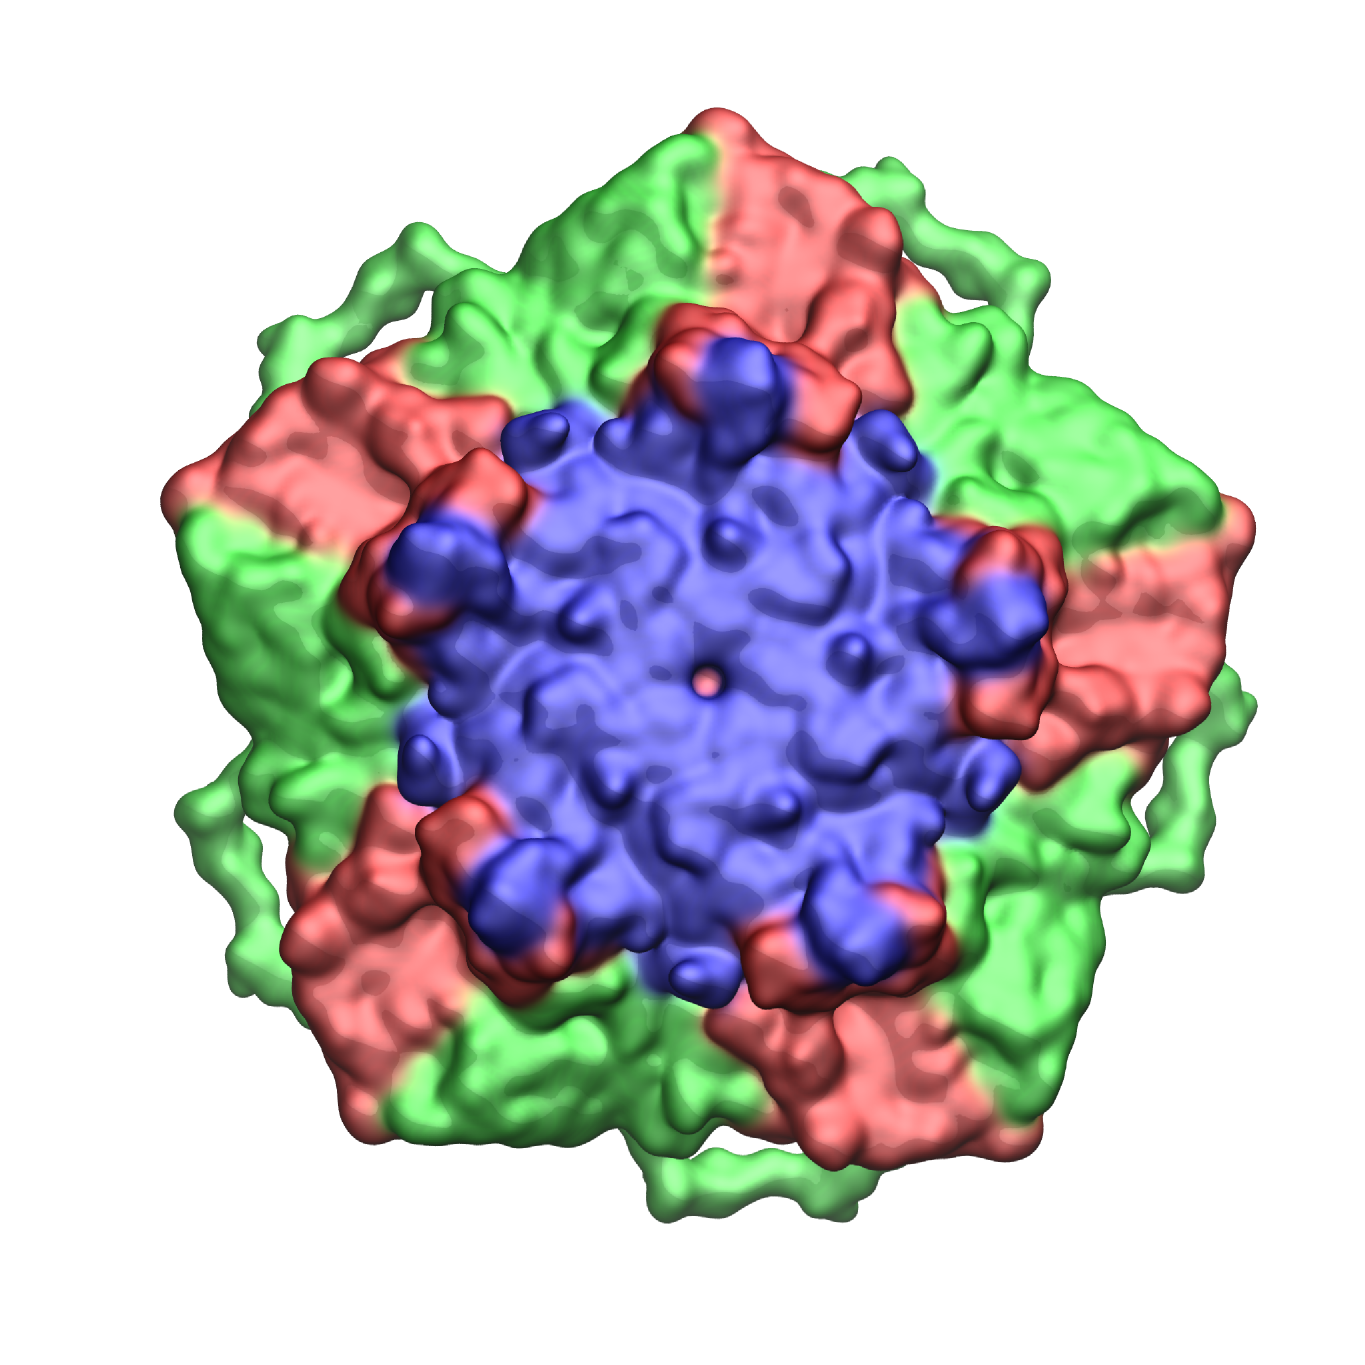
\includegraphics[width=1\textwidth]{Figure/TrV_Pentamer_Ch4.png}
  \end{subfigure}
\hspace*{\fill}
\end{figure}
}

\only<2>{
\centering
\begin{figure}[ht]
  \centering
  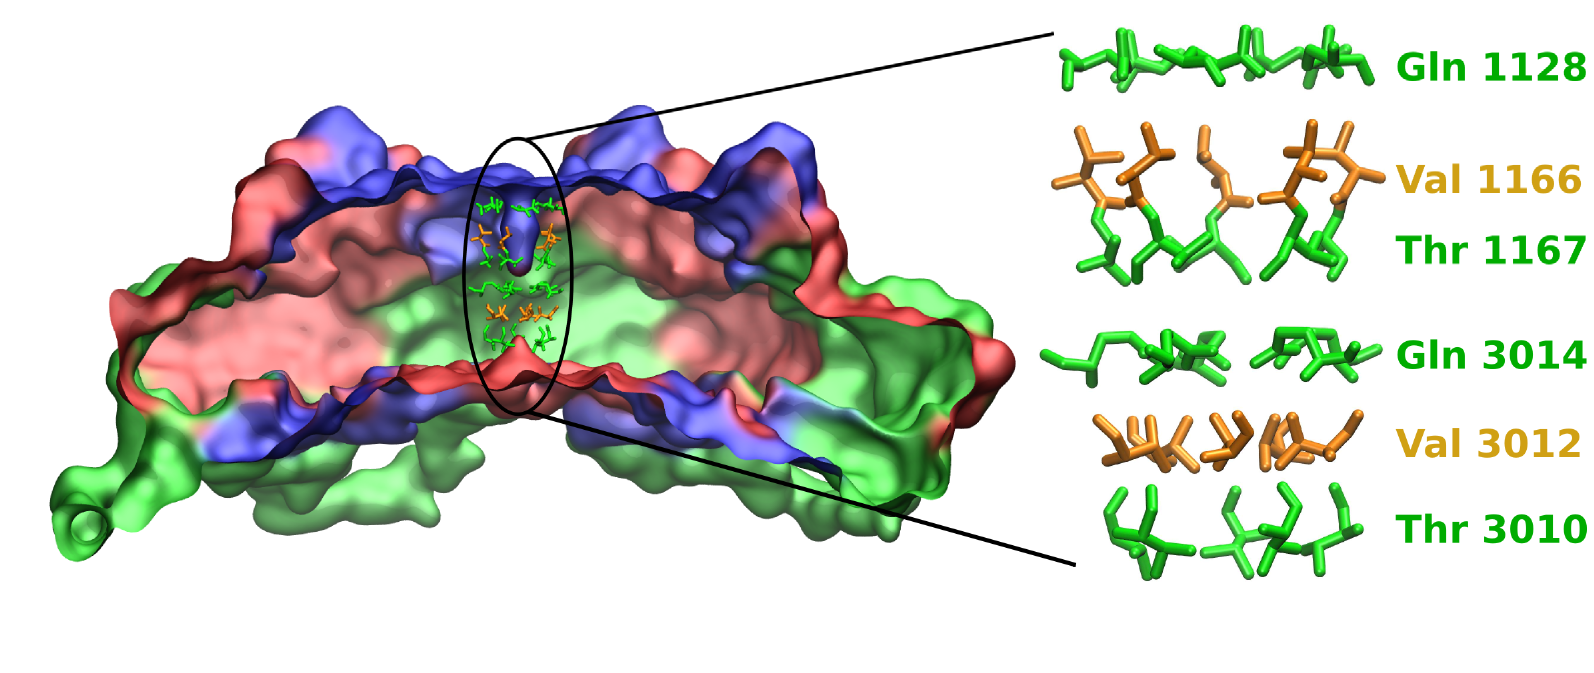
\includegraphics[width=1\textwidth]{Figure/TrV_Sideview_Pore.png}
\end{figure}
}

\end{frame}

\begin{frame}[t]{Objetivos}
\justifying
\begin{wrapfigure}{r}{0.4\textwidth}
\vspace{-0.5cm}
\Centering
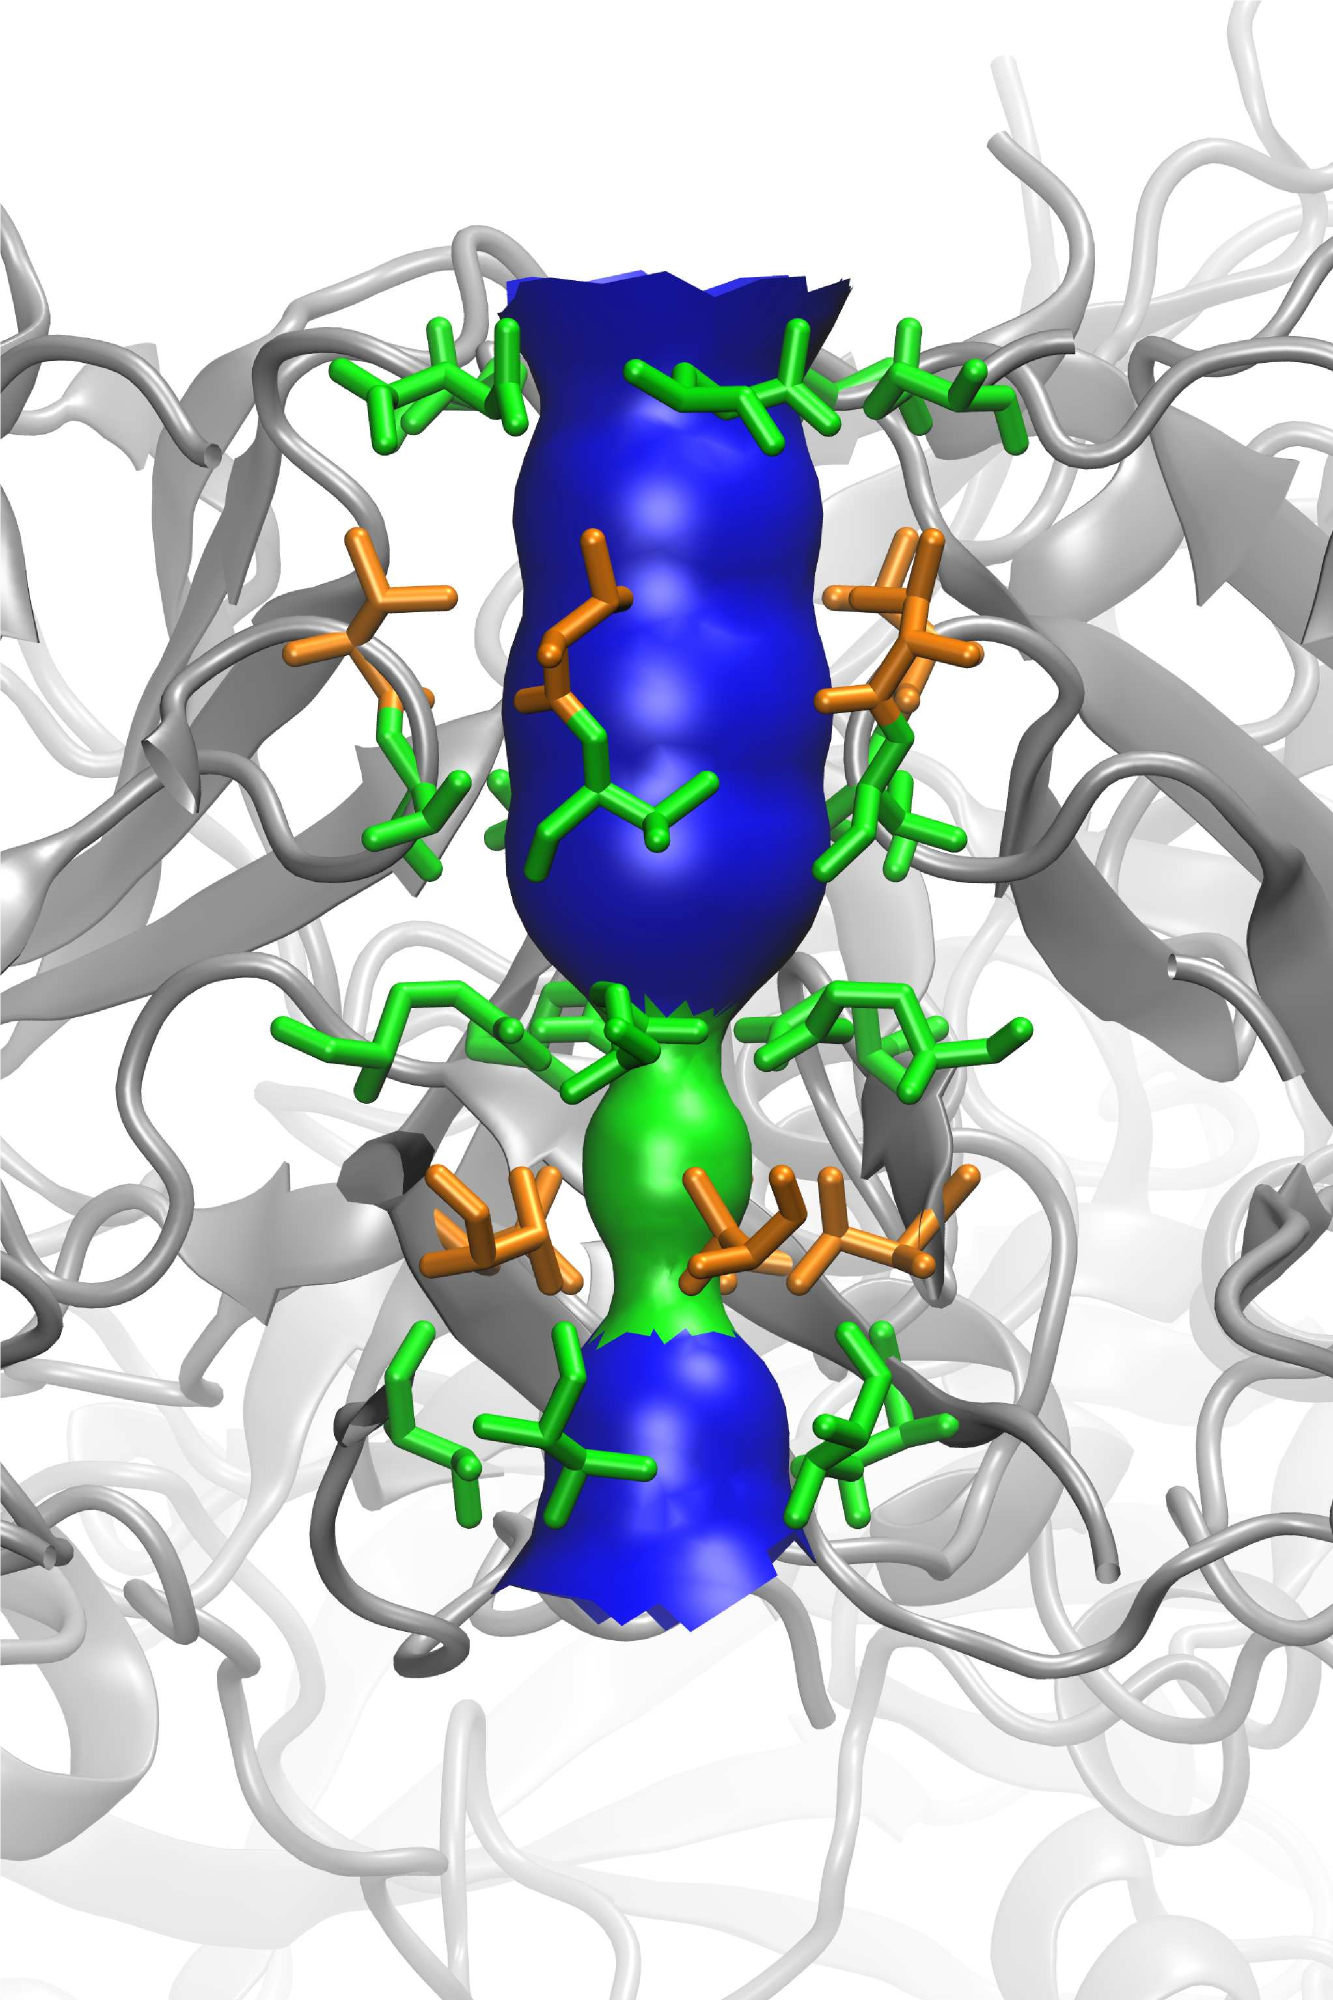
\includegraphics[width=0.35\textwidth]{Figure/TrV_SIdeview_Pore_2.png}
\end{wrapfigure}

El objetivo de esta tesis es lograr determinar, a partir de técnicas computacionales, el rol de la cavidad presente en el eje de simetría quíntuple en el virus del Triatoma.
\begin{itemize}
\justifying
\item[$\bullet$] Determinar si el poro de TrV tiene función de canal.
\item[$\bullet$] Determinar si el poro posee algún mecanismo de regulación de su apertura.
\item[$\bullet$] Determinar que tipo de moléculas son capaces de atravesarlo.
\item[$\bullet$] Determinar similitudes y diferencias entre la estructura del eje quíntuple con la estructura de otros virus pertenecientes al género.
\end{itemize}

\end{frame}

% These three lines create an automatically generated table of contents.
\begin{frame}[t]{}
  \tableofcontents
\end{frame}

\AtBeginSection[]{                              % Frame added before each section
  \frame<handout:0>{
    \tableofcontents[current]                   % Highlight current section/subsection
  }
}

\section{Introducción}

\begin{frame}[t]{Introducción}
\begin{itemize}
  \item Sistema de Estudio - TrV: Poro.
  \item Método - Simulación Computacional: Dinámica Molecular.
  \item Antecedentes (Kalko?).
\end{itemize}
\end{frame}


\begin{frame}[t]
\begin{itemize}
  \item Proteínas.
  \item Canales de proteínas.
  \item Virus.
  \item TrV.
  \item Hidrofobicidad.
\end{itemize}
\end{frame}


\begin{frame}[t]{Dinámica Molecular}

Integrador de Leap-Frog:
\begin{align*}
&x(t+\Delta t) = x(t) + v(t+\frac{1}{2}\Delta t){\Delta t} \nonumber \\
&v(t+\frac{1}{2}\Delta t) = v(t-\frac{1}{2}\Delta t) + a\Delta t
\end{align*}

\invisible<-1>{
Campo de Fuerzas:
\begin{multline*}
V = \sum\limits_{enlaces} \frac{k_{b,i}}{2} (l_i-l_{i0})^2 + \sum\limits_{angulos} \frac{k_{\theta,i}}{2} (\theta_i-\theta_{i,0})^2 + \sum\limits_{torsiones} \frac{\nu_n}{2} (1+cos(n\omega-\gamma)) \\
+ \sum\limits_{i=1} \sum\limits_{j=i+1} (
\tikzmarkin<3->[set fill color=red!10, set border color=red]{a}(0,-0.4)(0,0.4) 4\epsilon[(\frac{\sigma_{ij}}{r_{ij}})^{12}-(\frac{\sigma_{ij}}{r_{ij}})^6] \tikzmarkend{a}
+ \tikzmarkin<3->[set fill color=blue!10, set border color=blue]{b}(0,-0.4)(0,0.4) \frac{q_iq_j}{4\pi\epsilon_0r_{ij}} \tikzmarkend{b}
)
\end{multline*}
}

\begin{minipage}{0.4\textwidth}
\invisible<-1>{
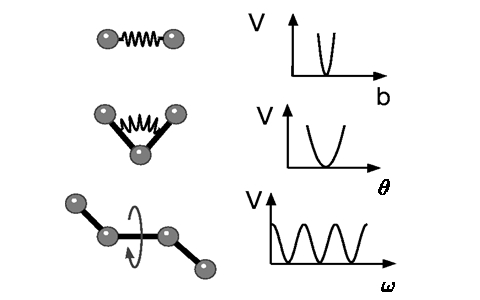
\includegraphics[width=\textwidth]{Figure/ff.jpg}
}
\end{minipage}
\begin{minipage}{0.59\textwidth}
\invisible<-2>{
  \vspace{-1.5cm}
  \begin{center}
  \begin{tabular}{cl}
  {\color{red} Potencial Coulombiano} \\ {\color{blue} Potencial de Lennard-Jones}
  \end{tabular}
  \end{center}
}
\end{minipage}

\end{frame}


\section{Poro en el eje quíntuple de TrV}
\begin{frame}[t]{Poro en el eje quíntuple de TrV}
\begin{itemize}
  \item Zhu et al.
  \item Hidratación
  \item Densmap y Radio del poro.
  \item Mutaciones.
\end{itemize}
\end{frame}

\begin{frame}[t]{Sistema a simular}

\begin{figure}[ht]
\vspace{-0.4cm}
\centering
\hspace*{\fill}
\begin{subfigure}[t]{.46\textwidth}
  \centering
  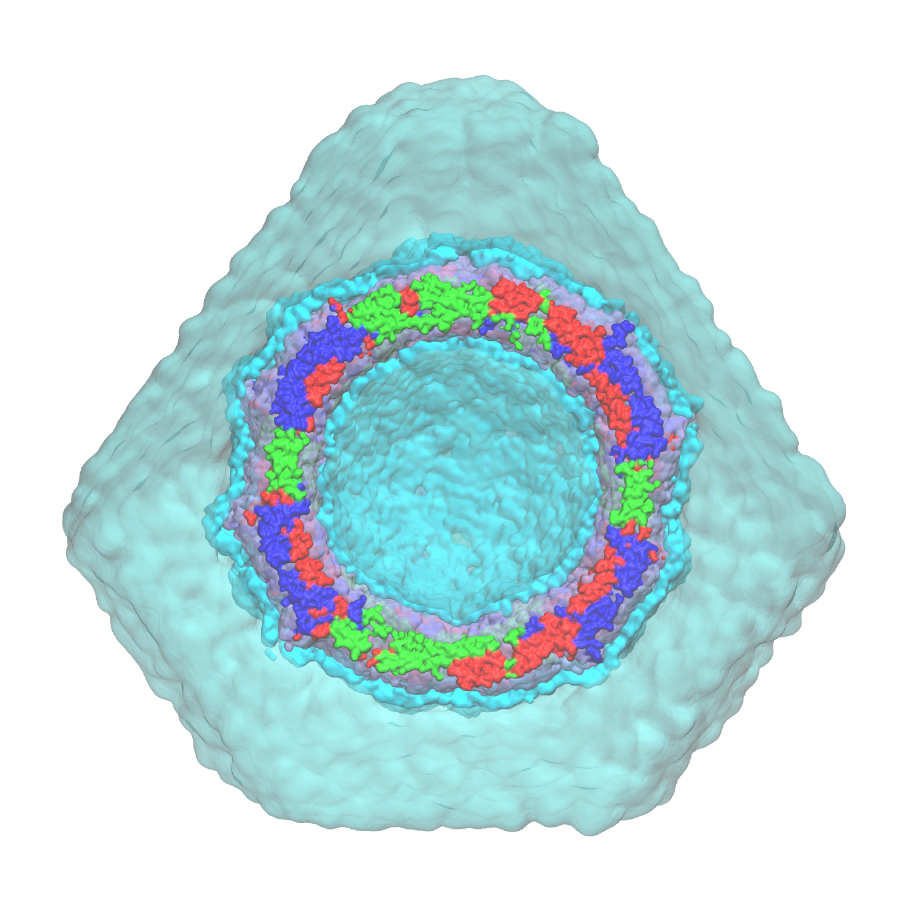
\includegraphics[width=1\textwidth]{Figure/TrV_Capsid_WaterBox.png}
  \caption{}
  \label{fig:trv_capsid_waterbox}
\end{subfigure}
\hspace*{\fill}
\begin{subfigure}[t]{.46\textwidth}
  \centering
  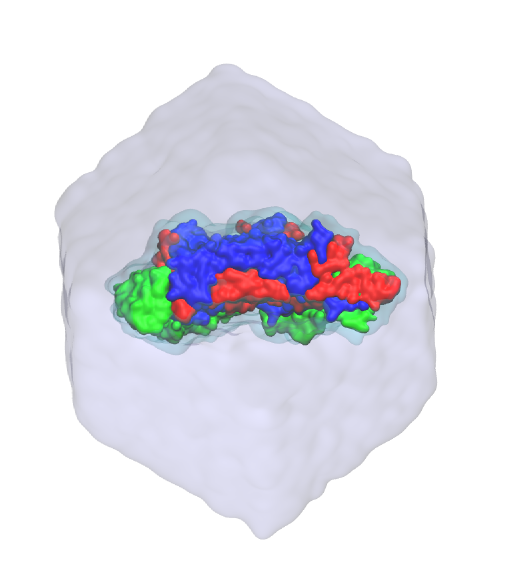
\includegraphics[width=1\textwidth]{Figure/TrV_Pentamer_WaterBox.png}
  \caption{}
  \label{fig:trv_pentamer_waterbox}
\end{subfigure}
\hspace*{\fill}
%\vspace{-10mm}
\caption*{\justifying Corte transversal del sistema de simulación, (a) cápside completa y (b) pentámero aislado. En azul, verde y rojo las superficies de las proteínas virales VP1, 2 y 3. Seguido de las capas de solvente SPC, WT4 y WLS representadas como superficies transparentes.}%
\end{figure}
\end{frame}


\begin{frame}[t]{Conclusión I}

\end{frame}


\section{Apertura de la Puerta}

\begin{frame}[t]{Perfil de Energía Libre en el poro de TrV}
\begin{itemize}
  \item Iones Mg$^{2+}$ y Mapa de Densidad Electrónico.
  \item PMF y Perfil de energía.
  \item DM con Mg, microsolvatación y Densmap.
\end{itemize}
\end{frame}


\begin{frame}[t]{Conclusión II}

\end{frame}


\section{Otros Virus}

\begin{frame}[t]{Puerta Hidrofóbica en otros Virus}
\begin{itemize}
  \item Mapa de Densidad de agua.
\end{itemize}
\end{frame}


\begin{frame}[t]{Conclusión III}

\end{frame}

\section{Conclusión}

\begin{frame}[t]{Conclusión}

\end{frame}


\begin{frame}[t]{Palabras Finales}

\end{frame}


\begin{frame}[t]{Agradecimientos}

\end{frame}


\end{document}